\documentclass[12pt]{article}
\usepackage[paper=letterpaper,margin=1.5cm]{geometry}
\usepackage{amsmath}
\usepackage{amssymb}
\usepackage{amsfonts}
\usepackage{mathtools}
%\usepackage[utf8]{inputenc}
%\usepackage{newtxtext, newtxmath}
\usepackage{lmodern}     % set math font to Latin modern math
\usepackage[T1]{fontenc}
\renewcommand\rmdefault{ptm}
%\usepackage{enumitem}
\usepackage[shortlabels]{enumitem}
\usepackage{titling}
\usepackage{graphicx}
\usepackage[colorlinks=true]{hyperref}
\usepackage{setspace}
\usepackage{subfigure} 
\usepackage{braket}
\usepackage{color}
\usepackage{tabularx}
\usepackage[table]{xcolor}
\usepackage{listings}
\usepackage{mathrsfs}
\usepackage{stackengine}
\usepackage{physics}
\usepackage{afterpage}
\usepackage{pdfpages}
\usepackage[export]{adjustbox}
\usepackage{biblatex}

\setstackEOL{\\}

\definecolor{dkgreen}{rgb}{0,0.6,0}
\definecolor{gray}{rgb}{0.5,0.5,0.5}
\definecolor{mauve}{rgb}{0.58,0,0.82}


\lstset{frame=tb,
  language=Python,
  aboveskip=3mm,
  belowskip=3mm,
  showstringspaces=false,
  columns=flexible,
  basicstyle={\small\ttfamily},
  numbers=none,
  numberstyle=\tiny\color{gray},
  keywordstyle=\color{blue},
  commentstyle=\color{dkgreen},
  stringstyle=\color{mauve},
  breaklines=true,
  breakatwhitespace=true,
  tabsize=3
}
\setlength{\droptitle}{-6em}

\makeatletter
% we use \prefix@<level> only if it is defined
\renewcommand{\@seccntformat}[1]{%
  \ifcsname prefix@#1\endcsname
    \csname prefix@#1\endcsname
  \else
    \csname the#1\endcsname\quad
  \fi}
% define \prefix@section
\newcommand\prefix@section{}
\newcommand{\prefix@subsection}{}
\newcommand{\prefix@subsubsection}{}
\renewcommand{\thesubsection}{\arabic{subsection}}
\makeatother
\DeclareMathOperator*{\argmin}{argmin}
\newcommand{\partbreak}{\begin{center}\rule{17.5cm}{2pt}\end{center}}
\newcommand{\alignbreak}{\begin{center}\rule{15cm}{1pt}\end{center}}
\newcommand{\tightalignbreak}{\vspace{-5mm}\alignbreak\vspace{-5mm}}
\newcommand{\hop}{\vspace{1mm}}
\newcommand{\jump}{\vspace{5mm}}
\newcommand{\R}{\mathbb{R}}
\newcommand{\C}{\mathbb{C}}
\newcommand{\N}{\mathbb{N}}
\newcommand{\G}{\mathbb{G}}
\renewcommand{\S}{\mathbb{S}}
\newcommand{\bt}{\textbf}
\newcommand{\xdot}{\dot{x}}
\renewcommand{\star}{^{*}}
\newcommand{\ydot}{\dot{y}}
\newcommand{\lm}{\mathrm{\lambda}}
\renewcommand{\th}{\theta}
\newcommand{\id}{\mathbb{I}}
\newcommand{\si}{\Sigma}
\newcommand{\Si}{\si}
\newcommand{\inv}{^{-1}}
\newcommand{\T}{^\intercal}
\renewcommand{\tr}{\text{tr}}
\newcommand{\ep}{\varepsilon}
\newcommand{\ph}{\varphi}
%\renewcomand{\norm}[1]{\left\lVert#1\right\rVert}
\definecolor{cit}{rgb}{0.05,0.2,0.45}
\addtolength{\jot}{1em}
\newcommand{\solution}[1]{

\noindent{\color{cit}\textbf{Solution:} #1}}

\newcounter{tmpctr}
\newcommand\fancyRoman[1]{%
  \setcounter{tmpctr}{#1}%
  \setbox0=\hbox{\kern0.3pt\textsf{\Roman{tmpctr}}}%
  \setstackgap{S}{-.9pt}%
  \Shortstack{\rule{\dimexpr\wd0+.1ex}{.9pt}\\\copy0\\
              \rule{\dimexpr\wd0+.1ex}{.9pt}}%
}

\newcommand{\Id}{\fancyRoman{2}}

% Enter the specific assignment number and topic of that assignment below, and replace "Your Name" with your actual name.
\title{STAT 31210: Homework 2}
\author{Caleb Derrickson}
\date{PUT DATE HERE}

\begin{document}
\onehalfspacing
\maketitle
\allowdisplaybreaks
{\color{cit}\vspace{2mm}\noindent\textbf{Collaborators:}} The TA's of the class, as well as Kevin Hefner, and Alexander Cram.

\tableofcontents

\newpage
\section{Problem 2.3}
Suppose that $f: G\rightarrow \R$ is a uniformly continuous function defined on an open subset $G$ of a metric space $X$. Prove that $f$ has a unique extension to a continuous function $\overline{f} : \Bar{G} \rightarrow \R$ defined on the closure $\Bar{G}$ of $G$. Show that such an extension need not exist if $f$ is continuous but not uniformly continuous on $G$.

\newcommand{\fbar}{\Bar{f}}

\partbreak
\begin{solution}

    Suppose we have a sequence $x_n \in \Bar{G}$. Since $\Bar{G}$ is closed, we can assume this sequence converges to the value $x \in \Bar{G}$. Define the extension $\fbar : \Bar{G} \rightarrow \R$ as $\fbar (x) = \lim_{n \rightarrow \infty} f(x_n)$. Note for all $n \in \N, x_n \in G$. And since $f$ is uniformly continuous on $G$, and also $x_n$ is Cauchy (it converges), $f(x_n)$ is then Cauchy. This is because for any sufficiently large $n, m \in \N$, we can make $d(x_n, x_m)$ arbitrarily small, i.e. less than some $\ep > 0$. $f$ is uniformly continuous, so for points close enough in the domain (take $x, y$), then their distance in the target space is also arbitrarily small. Therefore, for sufficiently large $N \in \N$ and $n, m \geq N$, we see that $d(x_n, x_m) < \ep$ for any $\ep > 0$. Therefore, $d(f(x_n), f(x_m)) < \ep$. \par

    \jump
    Note that the target space, $\R$, is complete, so stating $\fbar(x \in \Bar{G}) = \lim_{n\rightarrow \infty} f(x_n)$ is well defined. We need to show now that $\fbar$ is unique and uniformly continuous. 

    \tightalignbreak
    \begin{itemize}[-]
        \item \underline{$\fbar$ is unique.}

        \jump
        Since $\R$ is complete and $f(x_n)$ is Cauchy, then the sequence has a limit, so this is well defined. If $a, b \in \R$, and $a = \lim_{n \rightarrow \infty} \fbar(x_n) = b$, then by the triangle inequality, 
        \[d(a, b) \leq d(a, f(x_n)) + d(f(x_n), b).\]
        Since $f(x_n) \rightarrow a$ and $f(x_n) \rightarrow b$, these two distances will approach zero in the limit as $\ep \rightarrow 0$. Therefore, $d(a, b) \leq \ep \rightarrow 0$, so $d(a, b) = 0 \iff a = b$. Therefore, $\fbar$ is unique.

        \item \underline{$\fbar$ is uniformly continuous.}

        \jump
        Since $f$ is continuous, there exists a $\delta > 0$ such that for $d(x, y) < \delta / 3, \ d(f(x), f(y)) < \ep / 3$, for some $\ep > 0$, and for any $x, y \in \Bar{G}$. Since $\Bar{G}$ is closed, there exists sequences $x_n \in G, \ y_n \in G$ for which $x_n \rightarrow x$ and $y_n \rightarrow y$ as $n \rightarrow \infty$. Explicitly, we see when $n \geq N_1 \in \N$, we can have $d(x_n, x) < \delta / 3$ and $d(y_n, y) < \delta / 3$. \par

        \jump
        When $n \geq N_1$, we see $d(x_n, y_n) \leq d(x_n, x) + d(x, y) + d(y, y_n)$ by the triangle inequality. These can all be made less than $\delta / 3$, therefore $d(x_n, y_n) < \delta$. This will imply that their distances under the transformation can be made arbitrarily small. In this case, we let $d(f(x_n), f(y_n)) < \ep / 3$. \par

        \jump
        Since $f(x_n)$ and $f(y_n)$ are both Cauchy sequences in $\R$, we see that $f(x_n) \rightarrow \fbar(x)$ and $f(y_n) \rightarrow \fbar(y)$. Therefore, there exists an $\N_2 \in \N$ such that, when $n \geq N_2$, implies both $d(f(x_n), \fbar(x))$ and $d(f(y_n), \fbar(y)$ can be made less than $\delta / 3$. Choose $N = \max \{ N_1, N_2 \}$. Therefore, for any $n \geq N$, 
        \[d(\fbar(x), \fbar(y)) \leq d(\fbar(x), f(x_n)) + d(f(x_n), f(y_n)) + d(f(y_n), \fbar(y)).\]
        All terms on the right hand side were shown to be less than $\ep / 3$. Therefore, $d(\fbar(x), \fbar(y)) < \ep$, implying $\fbar$ is uniformly continuous.
    \end{itemize}
\end{solution}

\newpage
\section{Problem 2.6}
Show that the space $C([a, b])$ equipped with the $L^1$-norm $\norm{\cdot}_1$ defined as 
\[\norm{f}_1 = \int_a^b |f(x)| \ dx\]
is incomplete. Show that if $f_n \rightarrow f$ with respect to the sup-norm, then $f_n \rightarrow f$ with respect to $\norm{\cdot}_1$. Give a counterexample to show the converse is not true.
\partbreak
\begin{solution}

    \begin{itemize}[-]
        \item \underline{Incompleteness with respect to $\norm{\cdot}_1$.}

        \jump
        For $n \in \N$, consider the sequence of functions:
        \[
        f_n(x) = \begin{cases}
            1, & x \in [a, \frac{b - a}{2}]\\
            1 - \frac{n}{b - a}(x - \frac{b - a}{2}), &x \in (\frac{b - a}{2},  \frac{b - a}{2} + \frac{b - a}{n}]\\
            0, & x \in (\frac{b - a}{2} + \frac{b - a}{n}, b]
        \end{cases}
        \]
        This sequence of funcitons converges to the step function, where we ``step down" from 1 to zero at the midpoint $\frac{b -a}{2}$. Figure \ref{fig:p2.6.1} shows the function sequence for the first few $n$ values, as well as $\norm{f_n - f}_1$, where $f$ is the sequence limit. More explicitly, we can evaluate the difference integral as 
        \[
        \int_a^b |f_n(x) - f(x)| \ dx = \int_{\frac{b - a}{2}}^{\frac{b - a}{2} + \frac{b - a}{n}} 1 - \frac{n}{b - a} \Big(x - \frac{b - a}{2}\Big) \ dx = \frac{b - a}{2n} \rightarrow 0 \text{ as } n \rightarrow \infty. 
        \]
        It's easy to see that $f_n$ is a cauchy sequence of continuous functions over $[a, b]$. However, since the limit $f$ is not continuous, $C([a, b])$ is incomplete with respect to $\norm{\cdot}_1$. 
        

        \begin{figure}[!ht]
            \centering
            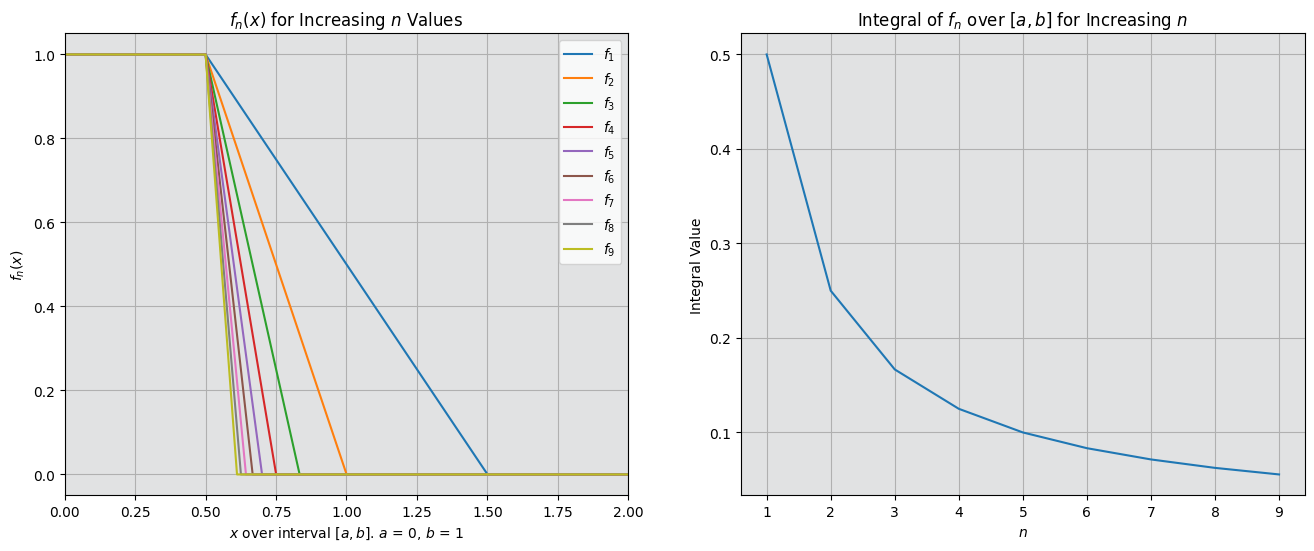
\includegraphics[width = 0.8\textwidth]{Images/Problem2.6.1.png}
            \caption{(Left) The sequence of functions $f_n$ described in Problem 2.6. The sequence ``steps down" from 1 to zero at the midpoint. (Right) The value of $\norm{f_n - f}_1$, where $\norm{\cdot}_1$ is the $L^1$ norm.}
            \label{fig:p2.6.1}
        \end{figure}
        \item \underline{Convergence wrt sup-norm implies convergence wrt $\norm{\cdot}_1$.}

        \jump
        Let $[a, b] = I$. We are given that $f_n \rightarrow f$ as $n \rightarrow \infty$ with respect to the sup norm. Thus, there exists $N \in \N$ such that when $n \geq N$ implies $\sup_{x \in I} |f_n(x) - f(x)| < \ep / (b - a)$. Thus, for any $x \in I$, $|f_n(x) - f(x)| < \ep / (b - a)$. Integrating both sides over $I$ yields
        \[\int_I |f_n(x) - f(x)| \ dx < \int_I \frac{\ep}{(b - a)} \ dx = \ep. \]
        The above inequality gives us $\norm{f_n(x) - f(x)}_1 \rightarrow 0$ as $n \rightarrow \infty$. 

        \item \underline{Counterexample of the converse.}
    \end{itemize}
\end{solution}
\clearpage

\newpage
\section{Problem 2.9}
Let $w : [0, 1] \rightarrow \R$ be a nonnegative, continuous function. For $f \in C([0, 1])$, define the weighted supremum norm by $\norm{f}_w = \sup_{0 \leq x \leq 1} \{ w(x)|f(x)|\}$.
\subsection{Problem 2.9, part 1}
If $w(x) > 0$ for $0 < x < 1$, show that $\norm{\cdot}_w$ is a norm on $C([0, 1])$.
\partbreak
\begin{solution}

    We just need to show the conditions for a norm hold. I will suppress the supremum bounds for legibility.
    \tightalignbreak
    \begin{itemize}[-]
        \item \underline{Absolute homogeneity.}

        \jump
        Suppose $\lm \in \R, f \in C([0, 1])$. Then, 
        \[\norm{\lambda f}_w = \sup \{ w(x)|\lm f(x)| \} = \sup \{ w(x)|\lm| |f(x)| \} = |\lm|\sup \{ w(x)|f(x)| \} = |\lm| \norm{f}_w\]

        \item \underline{Positive definiteness.}

        \jump
        If $\norm{f}_w = 0$, then $w(x)|f(x)| = 0$ for all $x \in [0, 1]$. Since $w(x) > 0$ for $0 < x < 1$, we can conclude $|f(x)| = 0$ for $x \in (0, 1)$. This can be extended to $[0, 1]$ since $f$ is continuous, so $f(0)$ and $f(1)$ cannot hold any nonzero value. Therefore, $f = 0$.  \par

        \jump
        If $f = 0$, then $\norm{f}_w = \sup \{ w(x) \cdot 0 \} = 0$ for all $x \in [0, 1]$. Therefore, $\norm{f}_1 = 0$. 

        \item \underline{Triangle Inequality.}

        \jump
        If $f, g \in C([0, 1])$, Then by the triangle inequality over $\R$,
        \begin{align*}
            \norm{f + g}_w &= \sup \{ w(x)|f(x) + g(x)| \} \leq \sup \{ w(x) (|f(x) + g(x)|)\} \\
            &\leq \sup \{w(x)|f(x)|\} + \sup\{w(x)|g(x)|\}\\ 
            &= \norm{f}_w + \norm{g}_w \\ 
            \implies \norm{f + g}_w &\leq \norm{f}_w + \norm{g}_w
        \end{align*}
    \end{itemize}
\end{solution}

\newpage
\subsection{Problem 2.9, part 2}
If $w(x) > 0$ for $x \in [0, 1]$, show that $\norm{\cdot}_w$ is equivalent to the usual sup-norm, corresponding to $w = 1$.
\partbreak
\begin{solution}

    By the definition in Chapter 5, we wish to ind a $c_1, c_2 > 0$ for which
    \[c_1\norm{f}_\infty \leq \norm{f}_w \leq c_2\norm{f}_\infty. \]
    Notice that 
    \[\norm{f}_w = \sup \{w(x)|f(x)|\} \leq \sup\{w(x)\}\sup\{|f(x)|\} = \sup\{w(x)\}\norm{f}_\infty\]
    So take $c_2 = \sup \{w(x)\}$. Next, consider $\inf\{w(x)\}$. Note that, since $w$ is a continuous function over a closed interval, then $w$ attains it maximum and minimum. Since $w(x) > 0$ for $x \in[0, 1]$, then $\min \{w(x)\} > 0$. Notice then, by the definition of minimum, 
    \[\inf\{w(x)\}\norm{f}_\infty = \sup\{\inf\{w(x)\}|f(x)|\} \leq \sup\{w(x)|f(x)|\} = \norm{f}_w\]
    So then take $c_1 = \min\{w(x)\}$. We have thus found $c_1, c_2$ for which the chain of inequalities is satisfied.    
\end{solution}

\newpage
\subsection{Problem 2.9, part 3}
Show that the norm $\norm{\cdot}_x$ corresponding to $w(x) = x$ is not equivalent to the usual sup-norm.
\partbreak
\begin{solution}

    From the argument I made in the previous part, since $w(0) = 0$, then $\min\{w(x): x \in [0, 1]\} = 0$. This then causes issues when passing into the supremum, so a similar argument cannot be made. \\
    \textbf{COME BACK TO THIS ONE.}
\end{solution}

\newpage
\subsection{Problem 2.13}
Consider the scalar initial value problem $\Dot{u}(t) = |u(t)|^\alpha, \ u(0) = 0$. Show that the solution is unique if $\alpha \geq 1$, but not if $0 \leq \alpha < 1$.
\end{document}